\section{Undirected Graphical Models}\label{sec:undirected_graphical_models}

\subsection{Factors}\label{sec:factors}

The characteristics of factors are defined as follows:
\begin{itemize}
\item Factors can not be directed in an undirected graphical model.
\item Factors subsumes both \emph{joint distribution} and \emph{conditional probability distribution}.
\item A joint distribution over $D$ is a factor over $D$. It specifies a real number for every assignment of values of $D$.
\item A conditional distribution $P(X|U)$ is a factor over $\{X\} \bigcup U$.
\item There are no constraints on a parameters in a factor.\marginnote{for example, in a joint distribution, the numbers must add up to $1$.}
\item A factor represents \emph{compatibility}/\emph{affinity} between the joining nodes.
\item A factor is only one contribution to the overall joint distribution.
\end{itemize}

\paragraph{Example: } Consider a fully connected graph over $\mathcal{X}$\marginnote{In a fully connected graph, there are no conditional independence.}.  Let all the variables be binary.  The we have:
\begin{itemize}
\item Each factor over an edge will have four parameters.
\item total number of parameters in the graph would be $4 \binom{n}{2}$.
\end{itemize}
\paragraph{Note} The number of parameters required to specify a joint distribution over $n$ binary variables is $2^n-1$.  The number of parameters available in an undirected graph is $4 \binom{n}{2}$. \[4 \binom{n}{2} <<< 2^n-1\]Therefore, pairwise factors do not have enough parameters to completely cover the joint distribution space. A more general representation can be obtained by allowing factors over an arbitrary subsets of variables.

\subsection {Factor Product}
Let $X$, $Y$, and $Z$ be three disjoint variable sets and let $\phi_1(X,Y)$ and $\phi_2(Y,Z)$ be two factors.  Then we define \emph{factor product} $\psi = \phi_1 \times \phi_2$, where $\psi:Val(X,Y,Z) \mapsto \mathbb{R}$.   $\psi(X,Y,Z)  = \phi_1(X,Y) \cdot \phi_2(Y,Z)$.  Note that the two factors are multiplied in a way that matches up the common part $Y$. 
\paragraph{Example} Let $\phi_1(A,B)$ and $\phi_2(B,C)$ be defined as follows:
\[
\begin{bmatrix}
a^1 & b^1 & 0.5 \\
a^1 & b^2 & 0.8 \\
a^2 & b^1 & 0.1 \\
a^2 & b^2 & 0 \\
a^3 & b^1 & 0.3 \\
a^3 & b^2 & 0.9
\end{bmatrix}
\cdot
\begin{bmatrix}
b^1 & c^1 & 0.5\\
b^1 & c^2 & 0.7\\
b^2 & c^1 & 0.1\\
b^2 & c^2 & 0.2
\end{bmatrix}
=
\begin{bmatrix}
a^1 & b^1 & c^1 & 0.5\cdot0.5=0.25 \\
a^1 & b^1 & c^2 & 0.5\cdot0.7=0.35 \\
a^1 & b^2 & c^1 & 0.8\cdot0.1=0.08\\
a^1 & b^2 & c^2 & 0.8\cdot0.2=0.16\\

a^2 & b^1 & c^1 & 0.05\\
a^2 & b^1 & c^2 & 0.07\\
a^2 & b^2 & c^1 & 0\\
a^2 & b^2 & c^2 & 0\\

a^3 & b^1 & c^1 & 0.15\\
a^3 & b^1 & c^2 & 0.21\\
a^3 & b^2 & c^1 & 0.09\\
a^3 & b^2 & c^2 & 0.18\\


\end{bmatrix}
\]

\subsection{Gibbs Distribution}
General notion of \emph{factors product} to define an undirected parametrization of a distribution.

\paragraph{Definition} A distribution $P_\phi$ is a Gibbs distribution, parametrized by a set of factors $\phi = \{ \phi_1(D_1),\ldots,\phi_k(D_k)\}$, if it is defined as follows:
\[P_\phi(X_1,\ldots,X_n) = \frac{1}{Z} \tilde{P}(X_1,\ldots,X_n)\] where
\[\tilde{P}(X_1,\ldots,X_n) = \phi_1(D_1) \times \phi_2(D_2) \times \ldots \times \phi_k(D_k)  \] and
\[ Z = \sum_{X_1,\ldots, X_k} \tilde{P}(X_1,\ldots,X_n) = \text{partition function}\]

\newthought{To map Gibbs distribution to a graph} we inspect the scope of the factors contained in the parametrization.  For example if the scope contain both $X$ and $Y$, then we will introduce an edge between $X$ and $Y$ nodes.

\paragraph {Markov network factorization} We say that a distribution $P_\phi$ with $\phi = \{\phi_1(D_1),\ldots,\phi_k(D_K)\}$ \emph{factorizes} over a \emph{markov network} $\mathcal{H}$ if each $D_k (k=1,\ldots, K)$ is a complete sub-graph of $\mathcal{H}$.

\paragraph {Clique potentials} The factors that parametrize a Markov network are often called \emph{clique potentials}.  Note that
\begin{itemize}
\item Every complete sub-graph is a subset of some (maximal) clique.  Therefore, we can reduce the number of factors in our parametrization by allowing factors only for maximal cliques. Let $C_1,\ldots,C_k$ be the cliques in $\mathcal{H}$, then we can parametrize $P$ using a set of factors $\phi_1(C_1),\ldots,\phi_k(C_l)$.
\item Any factorization (in terms of complete sub-graph) can be converted into this form simply by assigning each factor to a clique that encompasses its scope. 
\item \emph{Clique potential} is then calculated by multiplying all the factors assigned to each clique.
\end{itemize}


\subsection{Pairwise Markov Networks}

\begin{marginfigure}
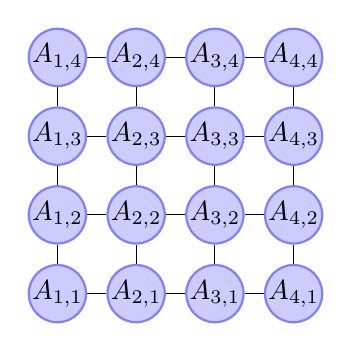
\begin{tikzpicture}
[mynode/.style={circle,draw=blue!50,fill=blue!20,thick, inner sep=0pt,minimum size=5mm}]

\node (n11) at ( 0,0) [mynode] {$A_{1,1}$};
\node (n12) at ( 0,1) [mynode] {$A_{1,2}$};
\node (n13) at ( 0,2) [mynode] {$A_{1,3}$};
\node (n14) at ( 0,3) [mynode] {$A_{1,4}$};

\node (n21) at ( 1,0) [mynode] {$A_{2,1}$};
\node (n22) at ( 1,1) [mynode] {$A_{2,2}$};
\node (n23) at ( 1,2) [mynode] {$A_{2,3}$};
\node (n24) at ( 1,3) [mynode] {$A_{2,4}$};

\node (n31) at ( 2,0) [mynode] {$A_{3,1}$};
\node (n32) at ( 2,1) [mynode] {$A_{3,2}$};
\node (n33) at ( 2,2) [mynode] {$A_{3,3}$};
\node (n34) at ( 2,3) [mynode] {$A_{3,4}$};

\node (n41) at ( 3,0) [mynode] {$A_{4,1}$};
\node (n42) at ( 3,1) [mynode] {$A_{4,2}$};
\node (n43) at ( 3,2) [mynode] {$A_{4,3}$};
\node (n44) at ( 3,3) [mynode] {$A_{4,4}$};

\foreach \from/\to in {n11/n21,n21/n31,n31/n41, n12/n22,n22/n32,n32/n42, n13/n23,n23/n33,n33/n43, n14/n24,n24/n34,n34/n44} 
	\draw (\from) -- (\to);

\foreach \from/\to in {n11/n12,n21/n22,n31/n32,n41/n42, n12/n13,n22/n23,n32/n33,n42/n43, n13/n14,n23/n24,n33/n34,n43/n44} 
	\draw (\from) -- (\to);

\end{tikzpicture}
\caption{A pairwise Markov network (MRF) structured as a grid.}
\end{marginfigure}

A pairwise Markov network over a graph $\mathcal{H}$ is associated with a set of node potentials $\{\phi(X_i): i=1,\ldots,n\}$ and a set of edge potentials $\{\phi(X_i, X_j): (X_i, X_j) \in \mathcal{H}\}$. The overall distribution is the normalized product of all of the potentials (both node and edge).
 \marginnote{A distribution where all of the factors are over single variables or pair of variables.}


\subsection{Reduced Markov Networks}
Conditioning a distribution on some assignment $u$ to some subset of variables$U$.
\marginnote{Conditioning a distribution corresponds to eliminating a ll entries in the joint distribution that are inconsistent with the event $U = u$, and renormalizing the remaining entries to sum to one.}

Let $\phi(Y)$ be a factor, and $U = u$ an assignment for $U \subseteq Y$.  We define the reduction of the factor $\phi$ to the context $U=u$, denoted by $\phi[U=u] = \phi[u]$, to be a factor over scope $Y' = Y - U$ such that:
\[ \phi[u](y', u) = \phi(y', u)\]






















